\documentclass[../report.tex]{subfiles}
\begin{document}


\chapter{\writingOK{Use case}} \label{cha:use_case}
This chapter shows a practical use case of using the newly implemented KHAPE library and demonstrate the security benefits.


\section{Context}

This section details use cases where using an aPAKE provide advantages over a classical authentication method.

\subsection{Online password manager}
Online password managers are among the most sensitive applications out there because the leakage of users’ data cascades into numerous compromised accounts on other services such as email accounts, social media, online banking.
Using an asymmetric PAKE for an online password manager makes a lot of sense because the client does not have to disclose its master password to the password manager host. In other words, the client does not have to trust the password manager host not to decrypt its personal data or leak the master password (or any other intentional or unintentional miss-handling).
In fact, multiple well-known online password manager such as iCloud Key Vault or 1Password uses an aPAKE (SRP).


\subsection{Other use cases}
More generally, using an aPAKE makes a lot of sense on applications where the server-side stored user data should not be visible to the server.  This is the case for applications where the server does not process the user's data. For example, online backup, secure vault, password managers, etc. This is achieved with encryption and so require an encryption key for the client.
Depending on the client, it is not feasible to store an additional symmetric key because it has to be securely stored --- e.g., with an HSM --- which cause problems of portability and key recovery. For example, for an online encrypted backup of a laptop or a smartphone, if the user loses its device, he cannot retrieve his online backup because the encryption key is stored on its lost device.
For portability, the encryption key is typically derived from the user's password --- the same password that he uses to authenticate with the server (you could require that the user input two different passwords but this is generally avoided because of bad user experience). Using a classical authentication method, the server store the user's encrypted sensitive data and also process the password in cleartext which is used to compute the encryption key. This void all the security of encrypting the sensitive data in the first place because the server --- or a malicious party who compromised the server --- could store the cleartext password, compute the encryption key and decrypt the sensitive user's data.
This is the reason why aPAKEs are very interesting in this case scenario. The server \textbf{never} see the user's password, so he cannot use it to decrypt user’s data.



% How to decrypt data (password manager's data) ?
% - password in KDF
% - using initial OPRF output
% - compute a new OPRF (different salt, same password ?)

% - Context/Introduction
% - Design
%   - Encrypted envelope (khape export key)
%   - Download/upload (khape session key)
%   - Auth/Register (no password leak)
%   - User's fonctionalities (CRUD)



% \section{Design}
% - multi user online password manager
% - Server store client's encrypted password registry
% - KHAPE export key is used to decrypt password registry
%     - derived from the hardened (slowhash) OPRF output
%         - an attacker that obtained the encrypted password registry and want to bruteforce the password has to request the server for every try since he doesn't know the server's secret salt.
% - Take full advantage of KHAPE, no password leakage, use export key
% - user talk to client, client talk to server



% What is it ? what can be done, what can it be used for
% usefulness of KHAPE -> no password leakage, export key
% encrypted registry and key derivation
% server endpoints
% client action (interaction)
% limitation / considerations

\section{Design}
This section describes the design of the use case: a multi-user online password manager.
The basic concept is that the server stores the encrypted user's data. 
Each client can only access his personal encrypted data from the server.

KHAPE is used for authentication between the client and the server. OPRF and SlowHash parameters are enabled to provide the highest level of security.


% The end user interact with a client which in turn communicate with the server.

\subsection{Encrypted user data}
Each user stores his encrypted user data on the server. This data include an Encrypted password registry and an Encrypted master key. Every encryption is computed by the authenticated encryption scheme XChaCha20-Poly1305.

The Encrypted password registry is a structure that contains the user's password. Passwords are double encrypted. The external structure --- the password registry --- is encrypted and then each individual password is also encrypted. Each encryption is performed with a different key, all derived from the master key.

The Encrypted master key is simply a key --- the Master key --- that is encrypted with another key --- the KHAPE's export key. 
One could derive the Master key from the KHAPE's export key but this means that if the user wants to change his authentication password, it is necessary to decrypt and re-encrypt every single password entry and the password registry with the new export key. This is not conceivable for a scalable password manager. Instead, in case of change in the authentication password, only the Master key is re-encrypted with the new export key. This idea is inspired from Bitwarden's online password manager design \cite{Bitwarden_Paper}.

% ProtectedRegistry:
% - ciphertext
% - nonce
% 
% Registry:
% - vec<PasswordEntry>
% - nonce
% 
% PasswordEntry:
% - label
% - username
% - ProtectePassword
% 
% ProtectedPassword:
% - ciphertext
% - nonce
% 
% Password:
% - data
% - nonce

\subsection{General process}
The figure \ref{fig:Online_password_manager} shows the entire process of reading a protected password from the authentication request to the password decryption.
\begin{enumerate}
 \item The user input his password in the client and the KHAPE authentication start (see section \ref{sec:khape_generic_algo} for details on the process).
 \item KHAPE authentication output a session key and an export key to the client. The session key is verified with the server. If the inputted password is invalid, no session key is outputted. An export key would still be outputted since it is not verifiable.
 \item Client request to download its encrypted data from the server using the session key as an authentication token. The server also stores the session key and can verify that the client has been successfully authenticated. An authentication token expires after 24 hours.
 \item If the authentication token is valid, the client receives his Encrypted master key and his Encrypted password registry.
 \item He decrypts the Encrypted master key with the KHAPE's export key to obtain his private key
 \item He computes two HKDF Expand with the Master key as an input and constant labels to obtain an External encryption key and an Internal encryption key
 \item He decrypts the Encrypted password registry with the External encryption key to obtain the Indexable password registry
 \item Now that the client has decrypted the external layer of the password registry, he remove the following value from memory: Export key, Master key, Encrypted master keys and Encrypted password registry. He still has to keep the Session key to communicate with the server and the external encryption key to re-encrypt the password registry upon modification.
 \item In the Indexable password registry each entry's label and username are in cleartext but the password is still unreadable. 
 \item When the user chooses to read a password entry, the client uses Internal encryption keys to compute an HKDF Expand with the entry's label and username as context. The result is a key that is unique for this password.
 \item The client finish by decrypting the encrypted password with the computed key. He obtains the readable password.
 \item After sending the cleartext password to the user, the client remove the cleartext password and the Individual password key from memory. This means that in IDLE the client only keeps Session key, External encryption keys, Internal encryption keys and Indexable password registry in memory.
\end{enumerate}

When the client adds, update or remove a password, he needs to update his Encrypted password registry and upload it to the server. This is done by computing an Individual password key from the Internal encryption key and the password entry's label and encrypting the password with this key. Then the password entry is added or updated in the password registry which is then encrypted with the External encryption key. The resulting ciphertext is sent to the server.

\begin{figure}[h]
 \centering
 \setlength{\fboxsep}{10pt}
 \setlength{\fboxrule}{1pt}
 \fbox{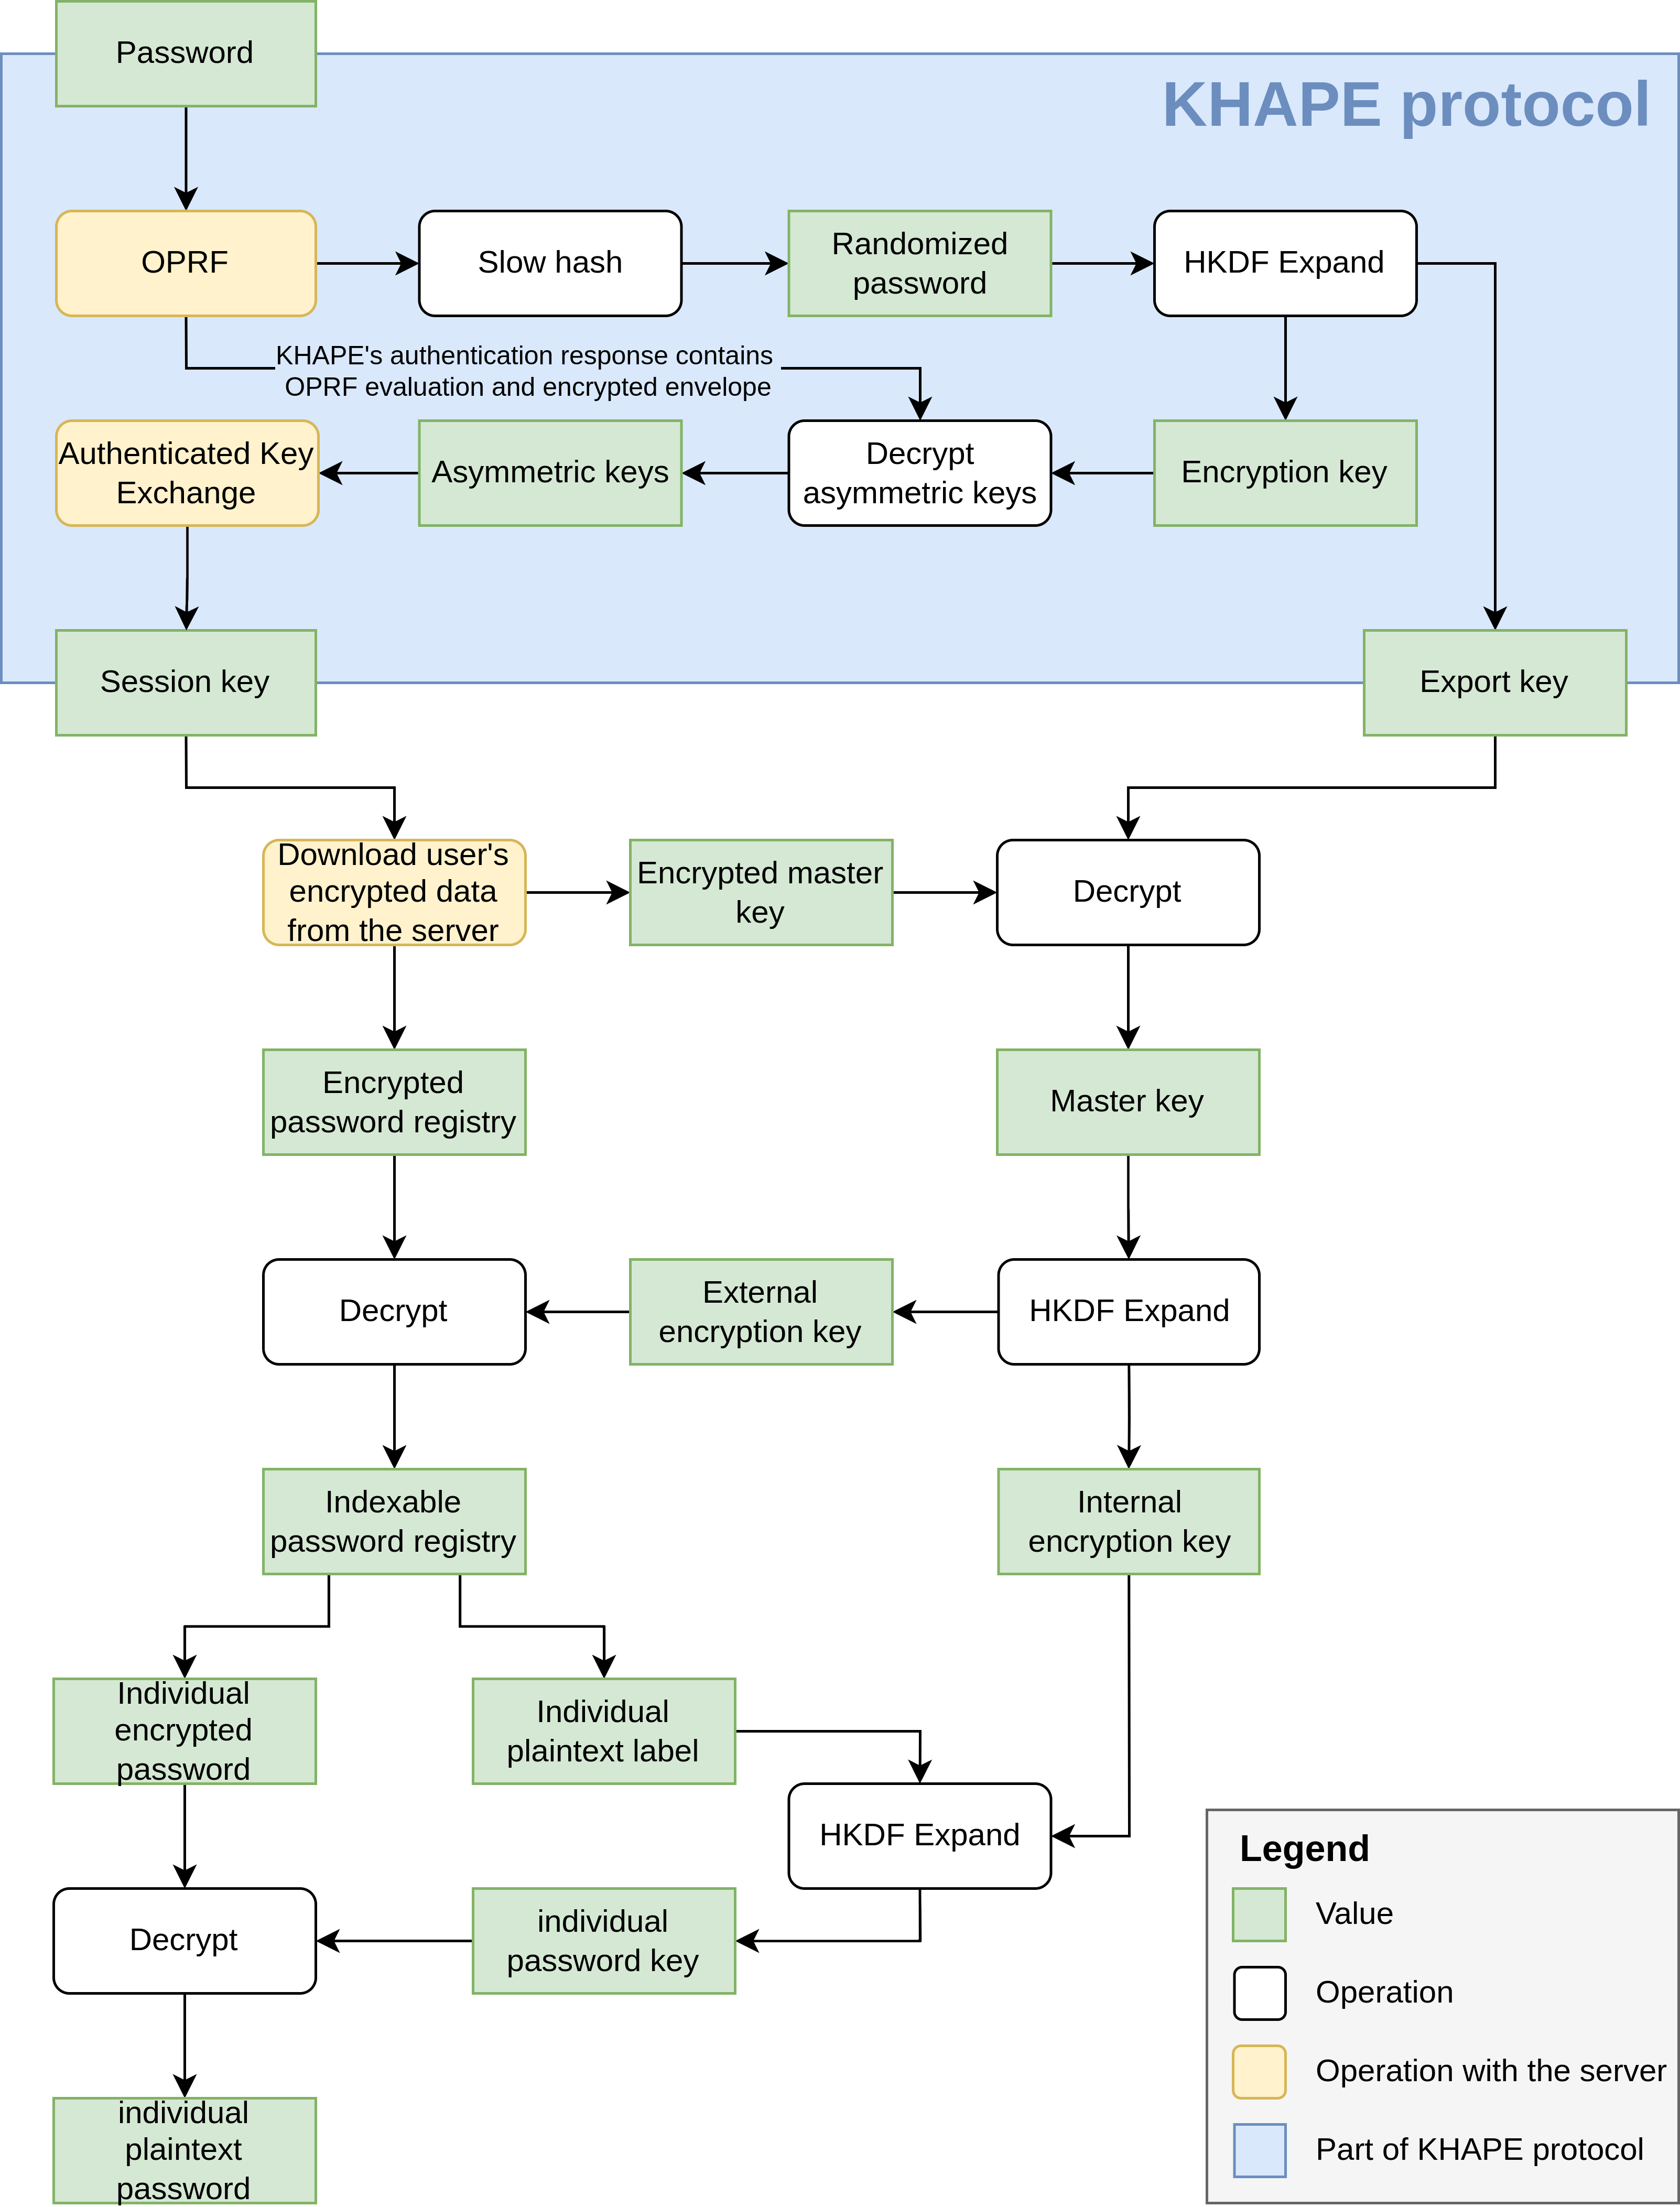
\includegraphics[width=\textwidth-22pt]{key-management.png}}
 \caption{Online password manager key derivation process to read a password.}
 \label{fig:Online_password_manager}
\end{figure}

\subsection{Server endpoints}
The server has only four endpoints:
\begin{itemize}
 \item Registration (KHAPE)
 \item Authentication (KHAPE)
 \item File download
 \item File upload
\end{itemize}
Registration and authentication are handled by KHAPE's protocol (see Section \ref{sec:khape_generic_algo}). Upon successful authentication, the client can use the outputted session key as an authentication token. He sends his session token with every request to prove to the server that he is authenticated. The session token expires after 24 hours.

File download and file upload allow the user to retrieve and commit his protected data from the server. The interactions between the client and the server are defined in the figure \ref{fig:usecase_download} for the file download endpoint and in the figure \ref{fig:usecase_upload} for the file upload endpoint.


\begin{figure}[h]
 \centering
 \setlength{\fboxsep}{10pt}
 \setlength{\fboxrule}{1pt}
 \fbox{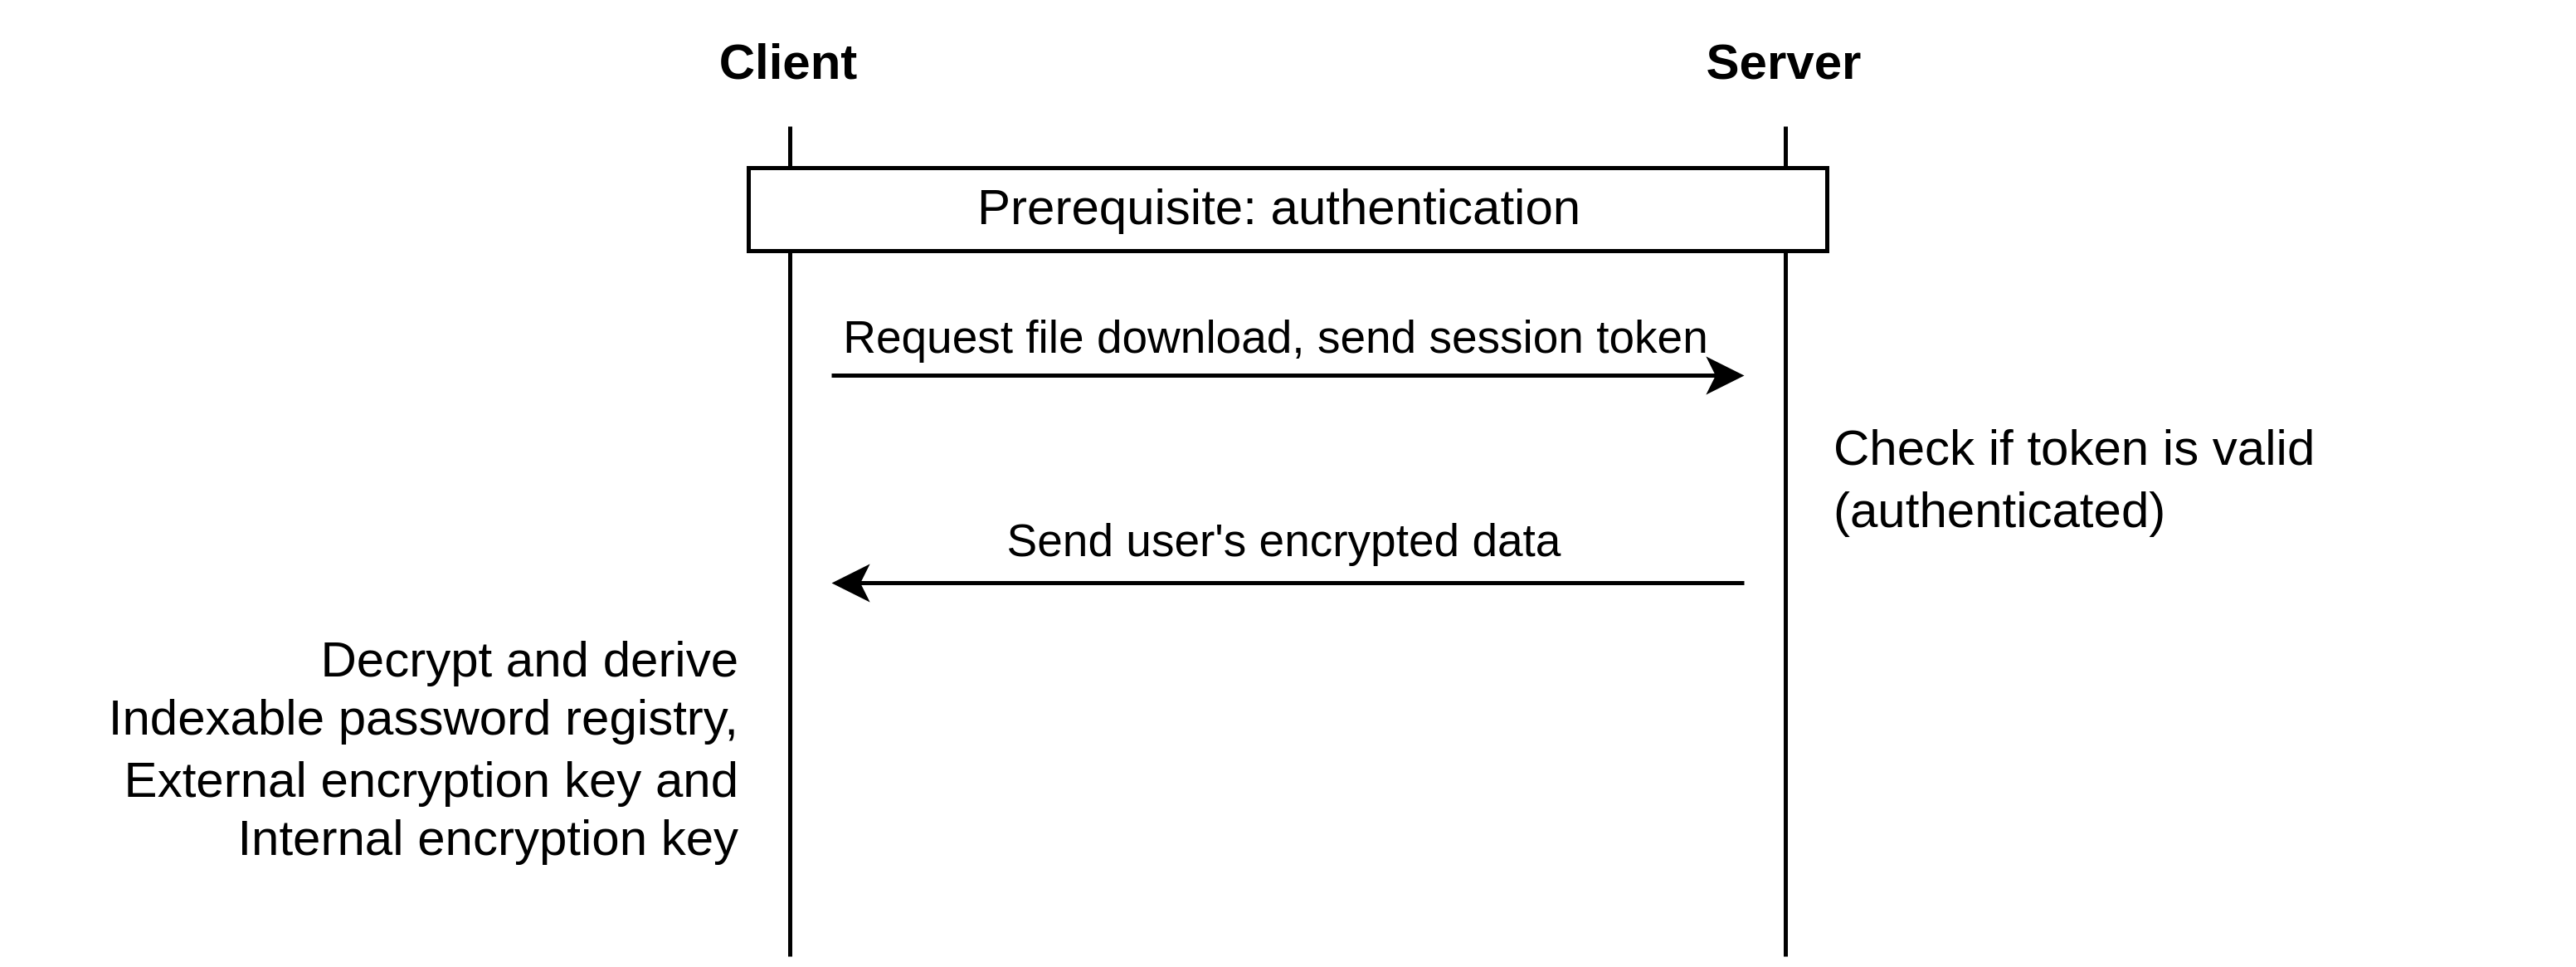
\includegraphics[width=\textwidth-22pt]{download.png}}
 \caption{Interaction between the client and the server for the file download endpoint.}
 \label{fig:usecase_download}
\end{figure}

\begin{figure}[h]
 \centering
 \setlength{\fboxsep}{10pt}
 \setlength{\fboxrule}{1pt}
 \fbox{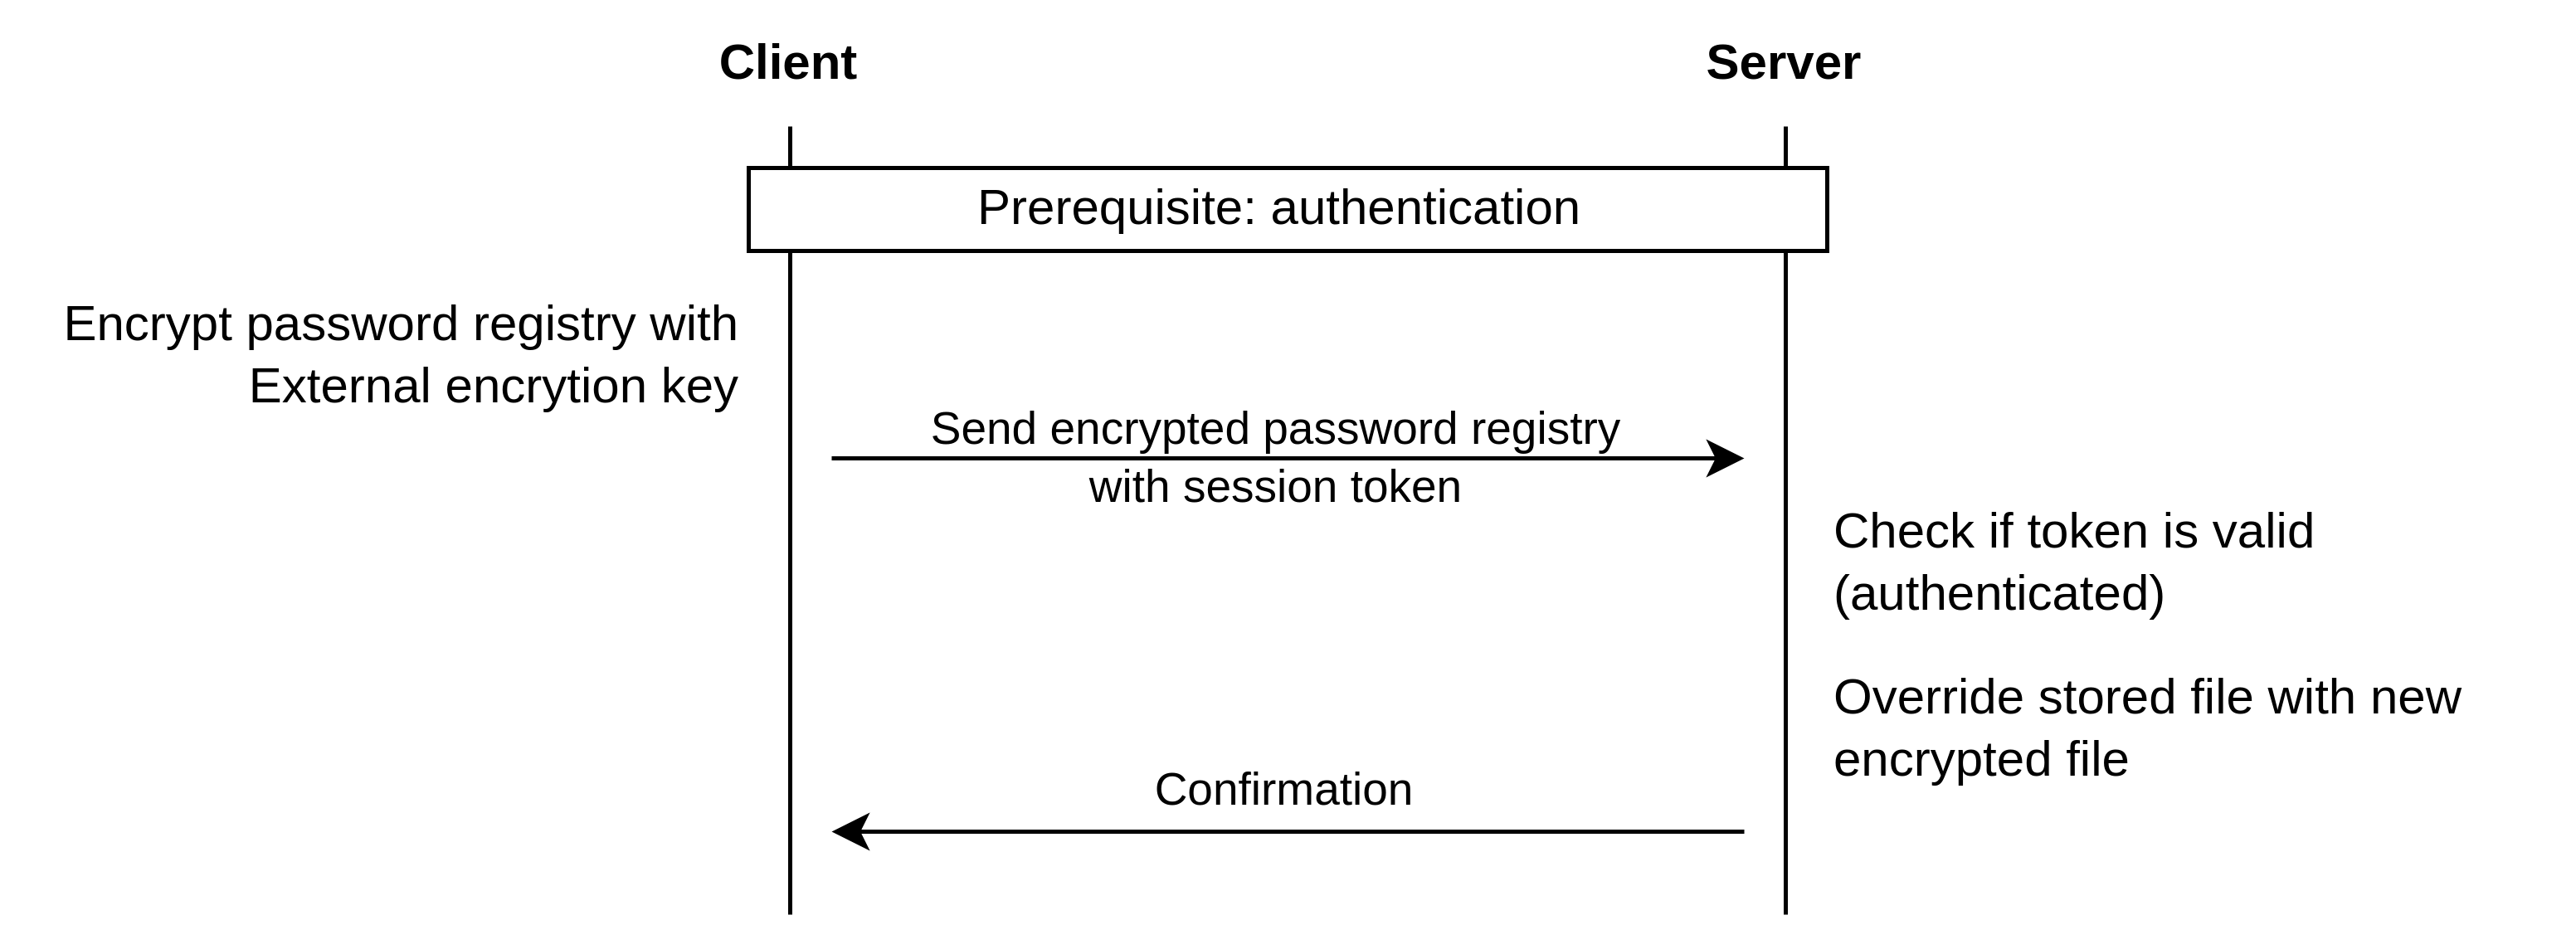
\includegraphics[width=\textwidth-22pt]{upload.png}}
 \caption{Interaction between the client and the server for the file upload endpoint.}
 \label{fig:usecase_upload}
\end{figure}


\subsection{Client actions}
The end user interacts with the client to access its passwords.
At client start, the user can either register or login.
After a successful registration, he still needs to login.

Upon successful authentication, the client automatically download the user's data file and the user can select one of the following actions :
\begin{itemize}
 \item Read a password
 \item Add a new password
 \item Modify a password
 \item Delete a password
\end{itemize}
For actions where the password registry is modified (adding, modifying or deleting a password), the password registry is re-encrypted by the client (with the External encryption key) and uploaded to the server.

The interactions between the user and the client are defined in the figure \ref{fig:usecase_read} for reading a password entry, in the figure \ref{fig:usecase_add} for adding a new password entry, in the figure \ref{fig:usecase_modify} for adding a modifying an existing password entry and in the figure \ref{fig:usecase_delete} for deleting a password entry.



\begin{figure}[h]
 \centering
 \setlength{\fboxsep}{10pt}
 \setlength{\fboxrule}{1pt}
 \fbox{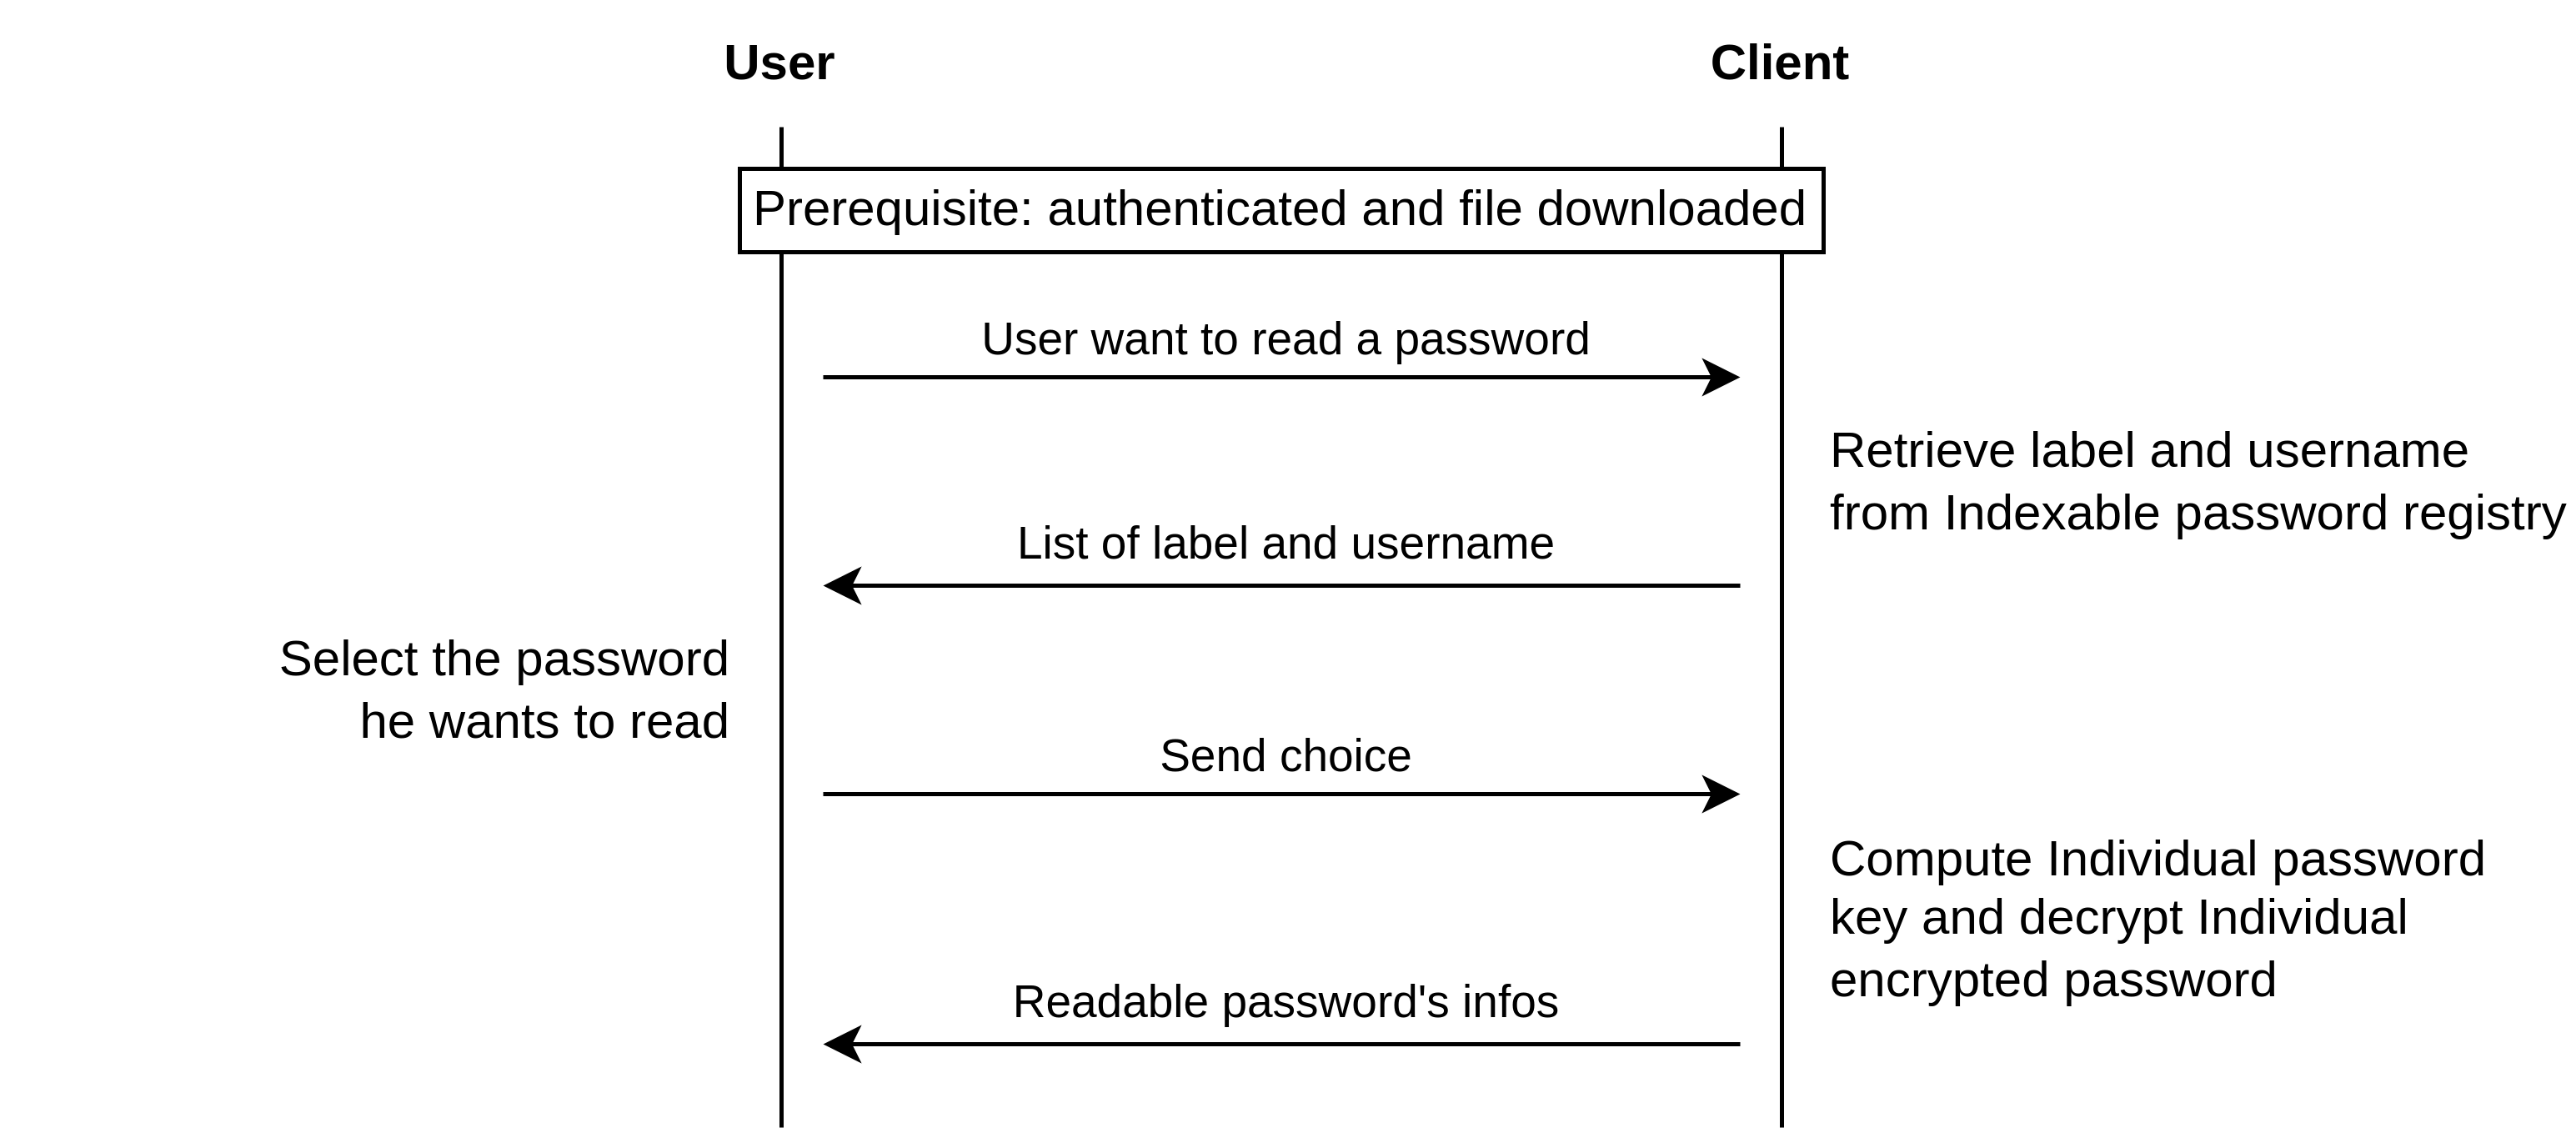
\includegraphics[width=\textwidth-22pt]{read.png}}
 \caption{Interaction between the user and the client for reading a password entry.}
 \label{fig:usecase_read}
\end{figure}

\begin{figure}[h]
 \centering
 \setlength{\fboxsep}{10pt}
 \setlength{\fboxrule}{1pt}
 \fbox{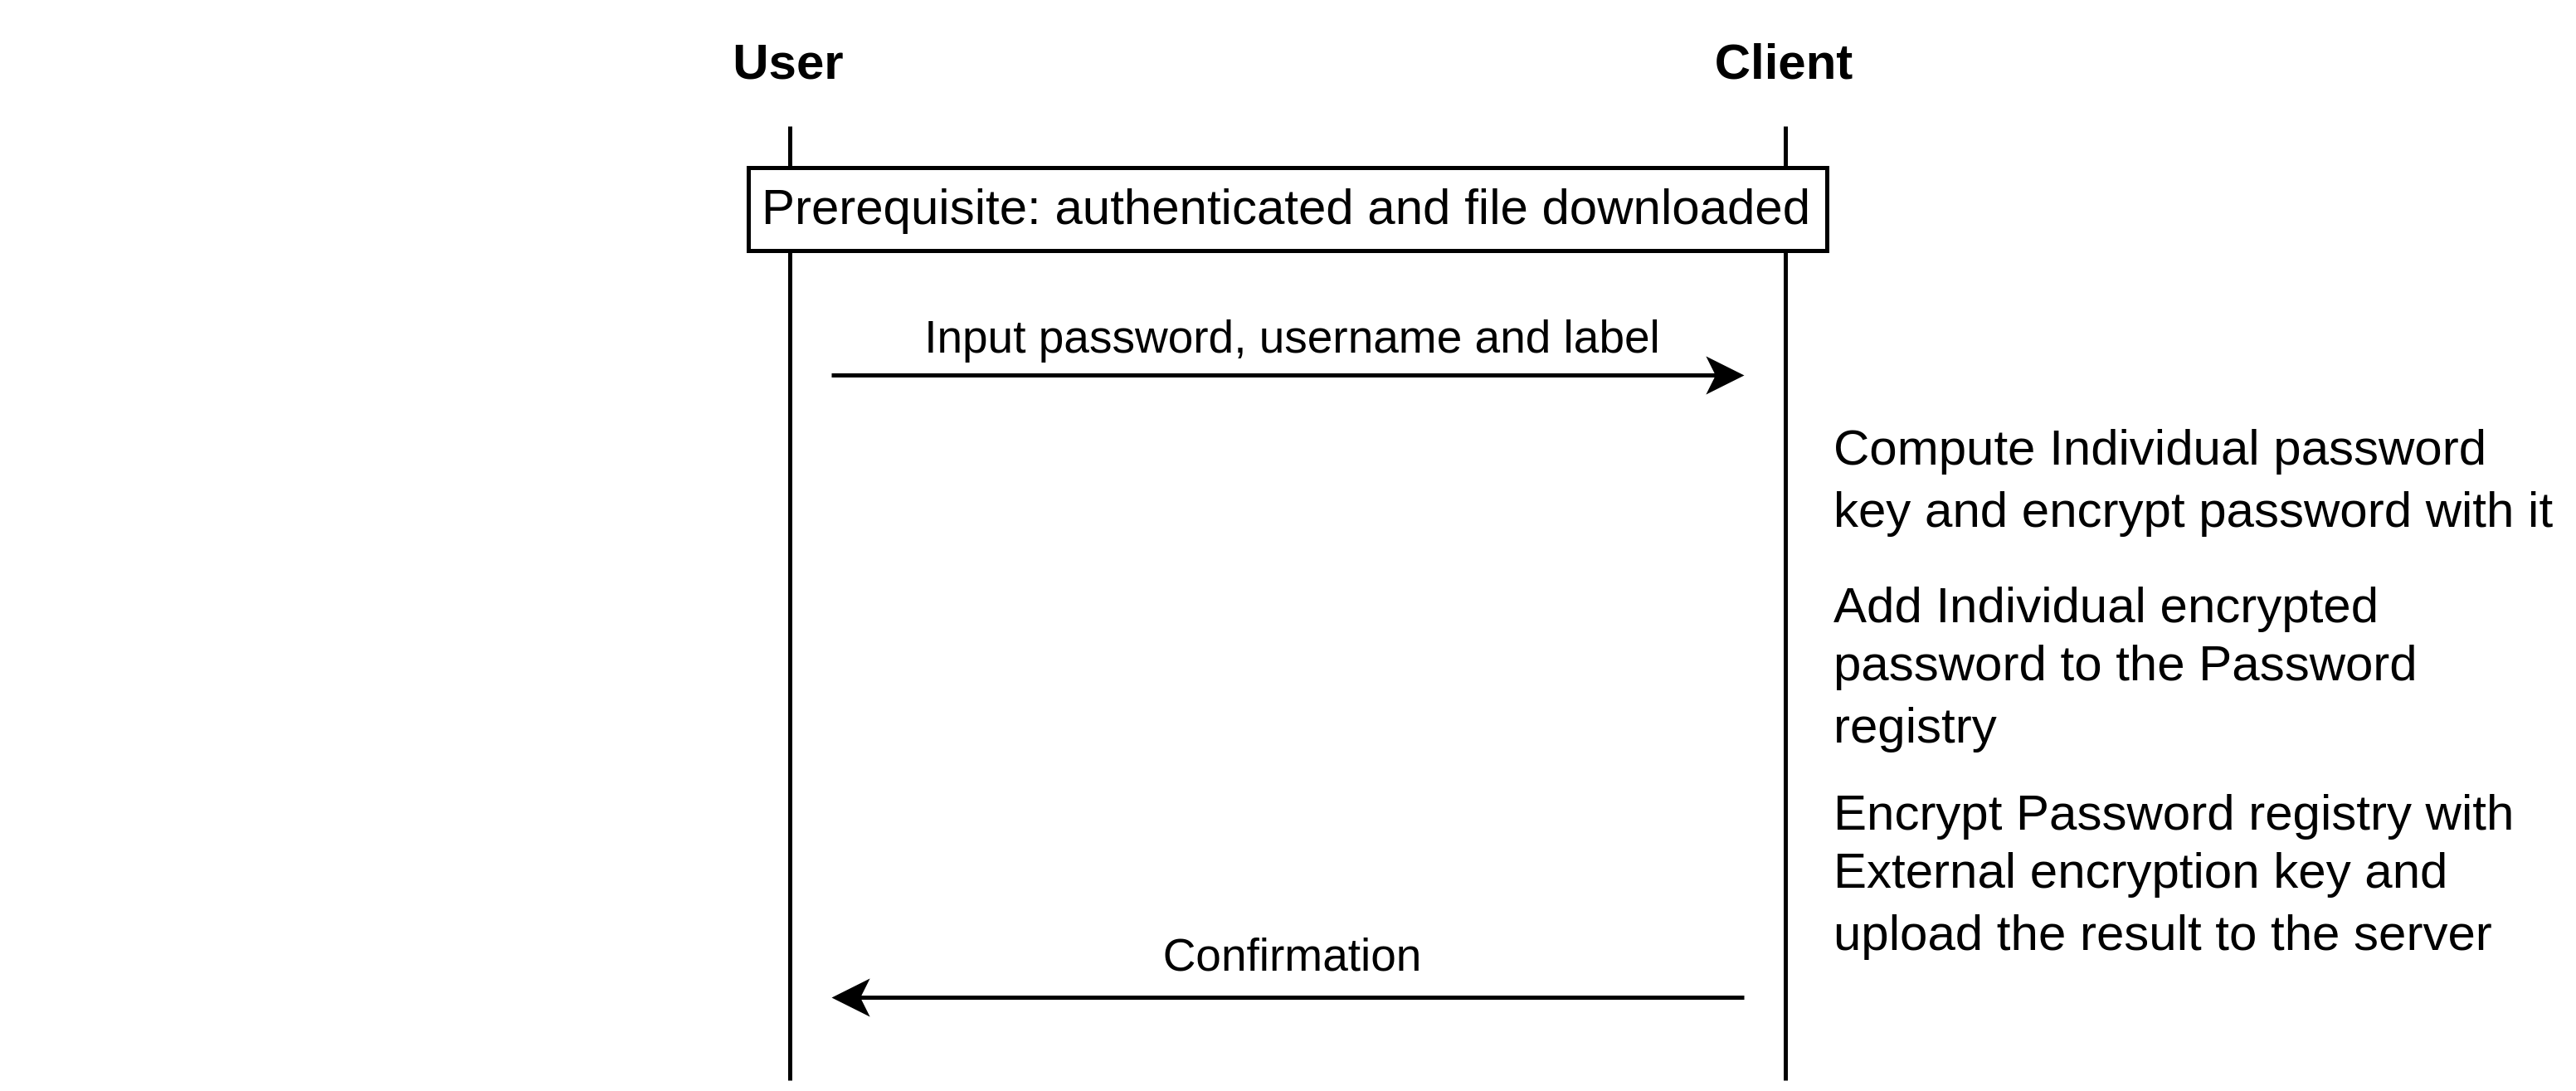
\includegraphics[width=\textwidth-22pt]{add.png}}
 \caption{Interaction between the user and the client for adding a new password entry.}
 \label{fig:usecase_add}
\end{figure}

\begin{figure}[h]
 \centering
 \setlength{\fboxsep}{10pt}
 \setlength{\fboxrule}{1pt}
 \fbox{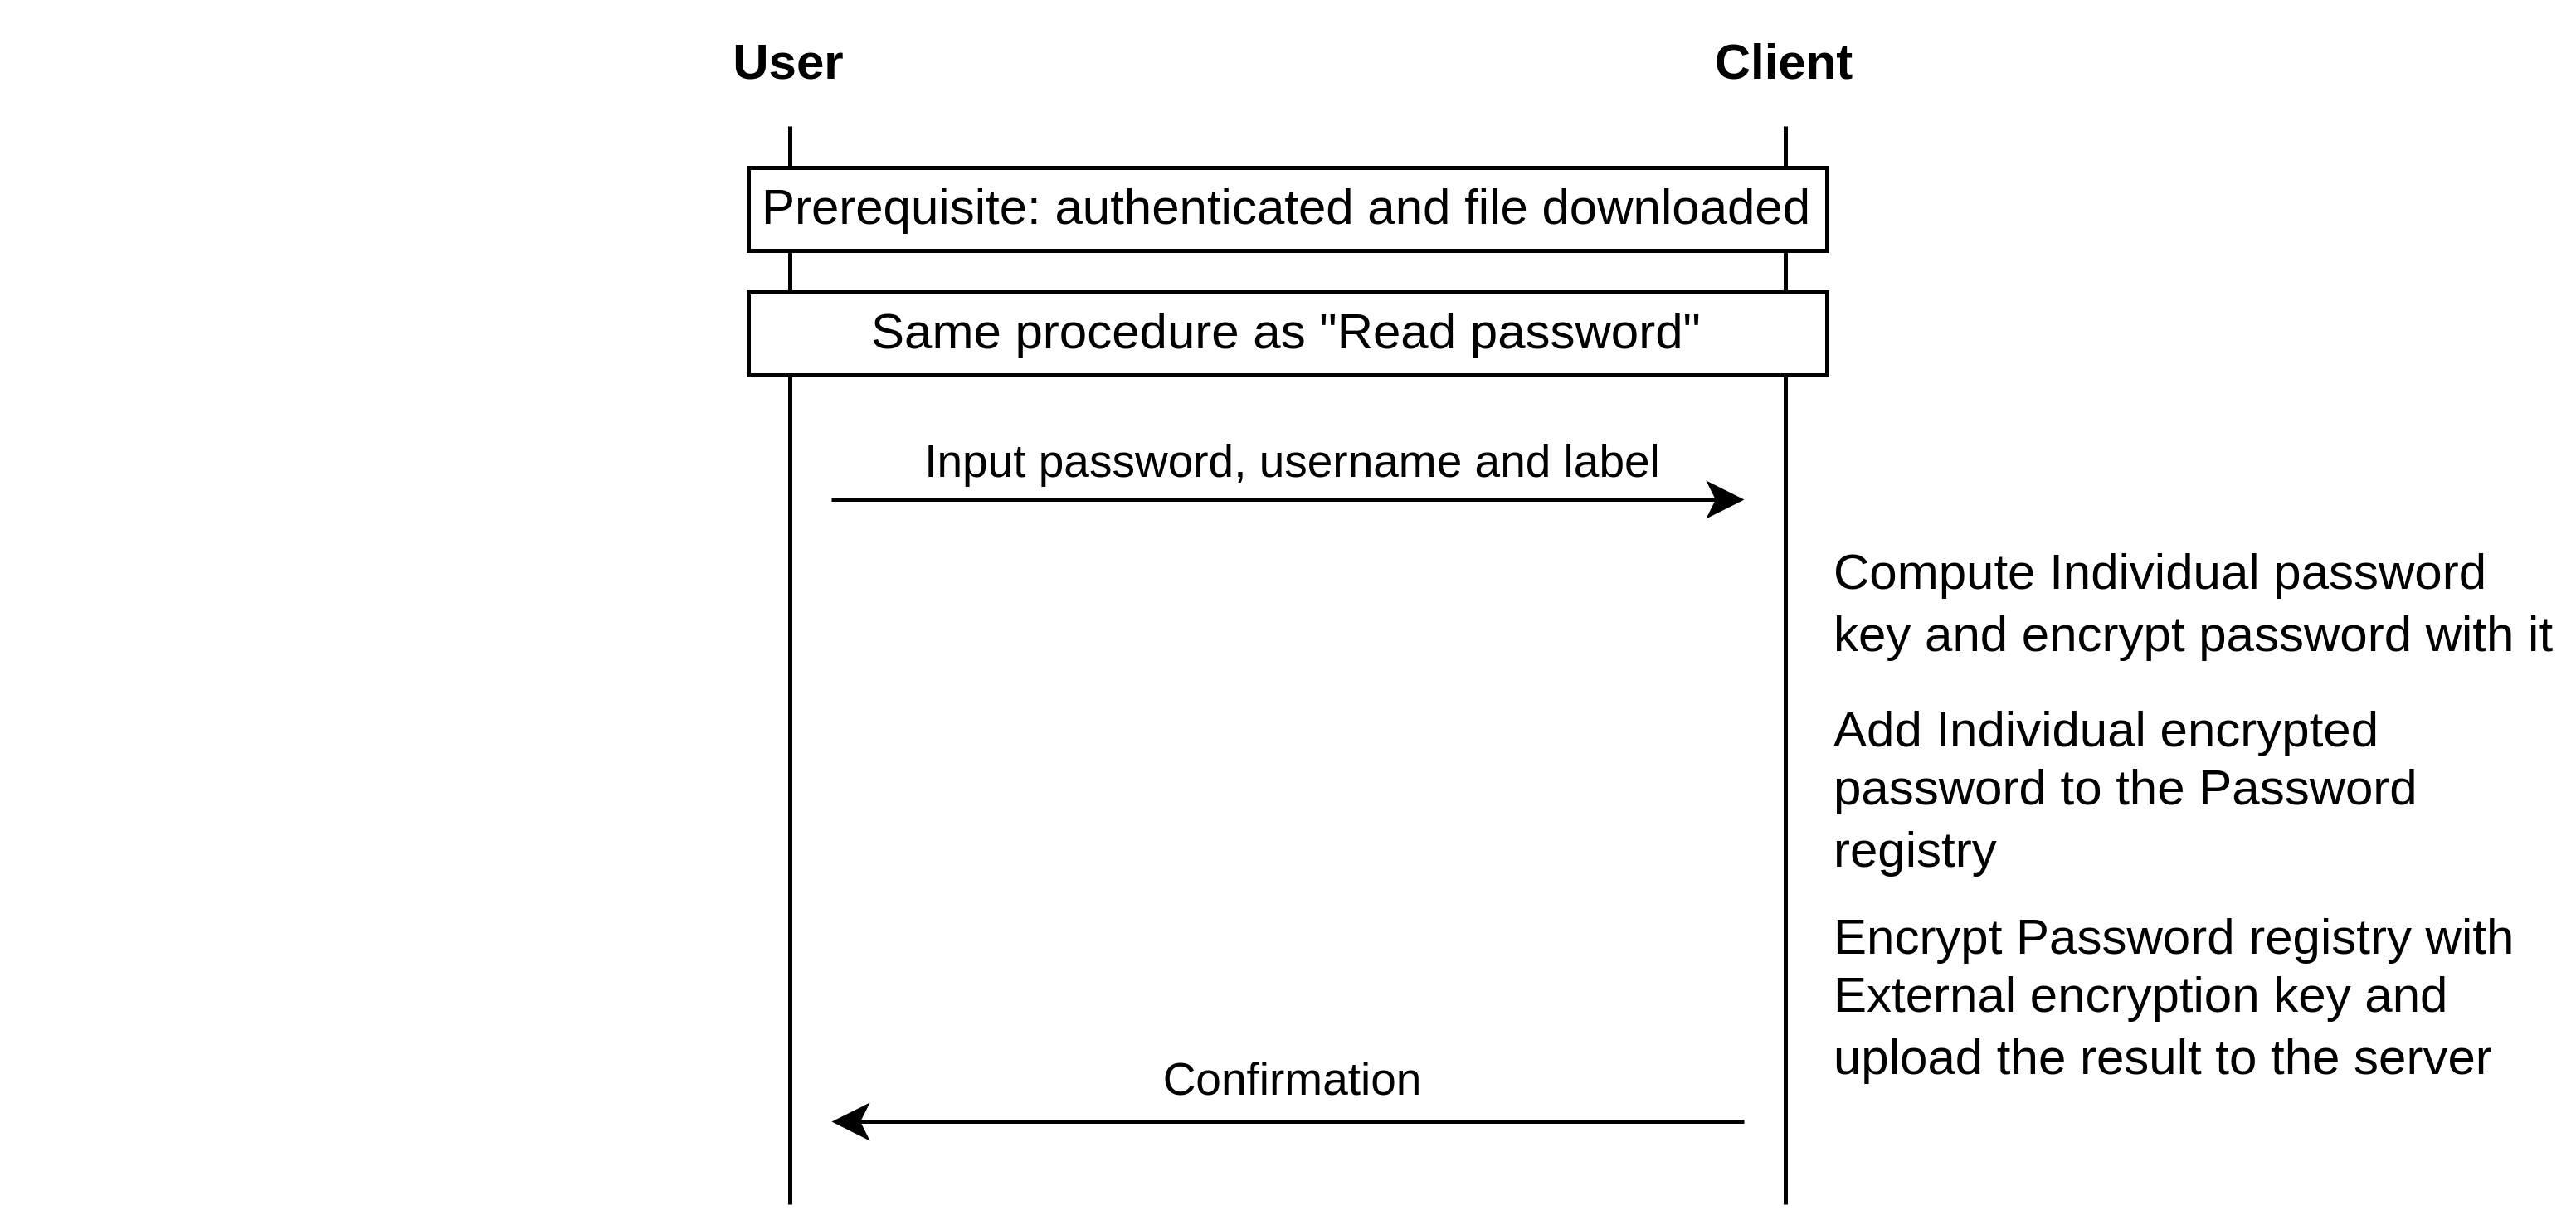
\includegraphics[width=\textwidth-22pt]{modify.png}}
 \caption{Interaction between the user and the client for modifying an existing password entry.}
 \label{fig:usecase_modify}
\end{figure}

\begin{figure}[h]
 \centering
 \setlength{\fboxsep}{10pt}
 \setlength{\fboxrule}{1pt}
 \fbox{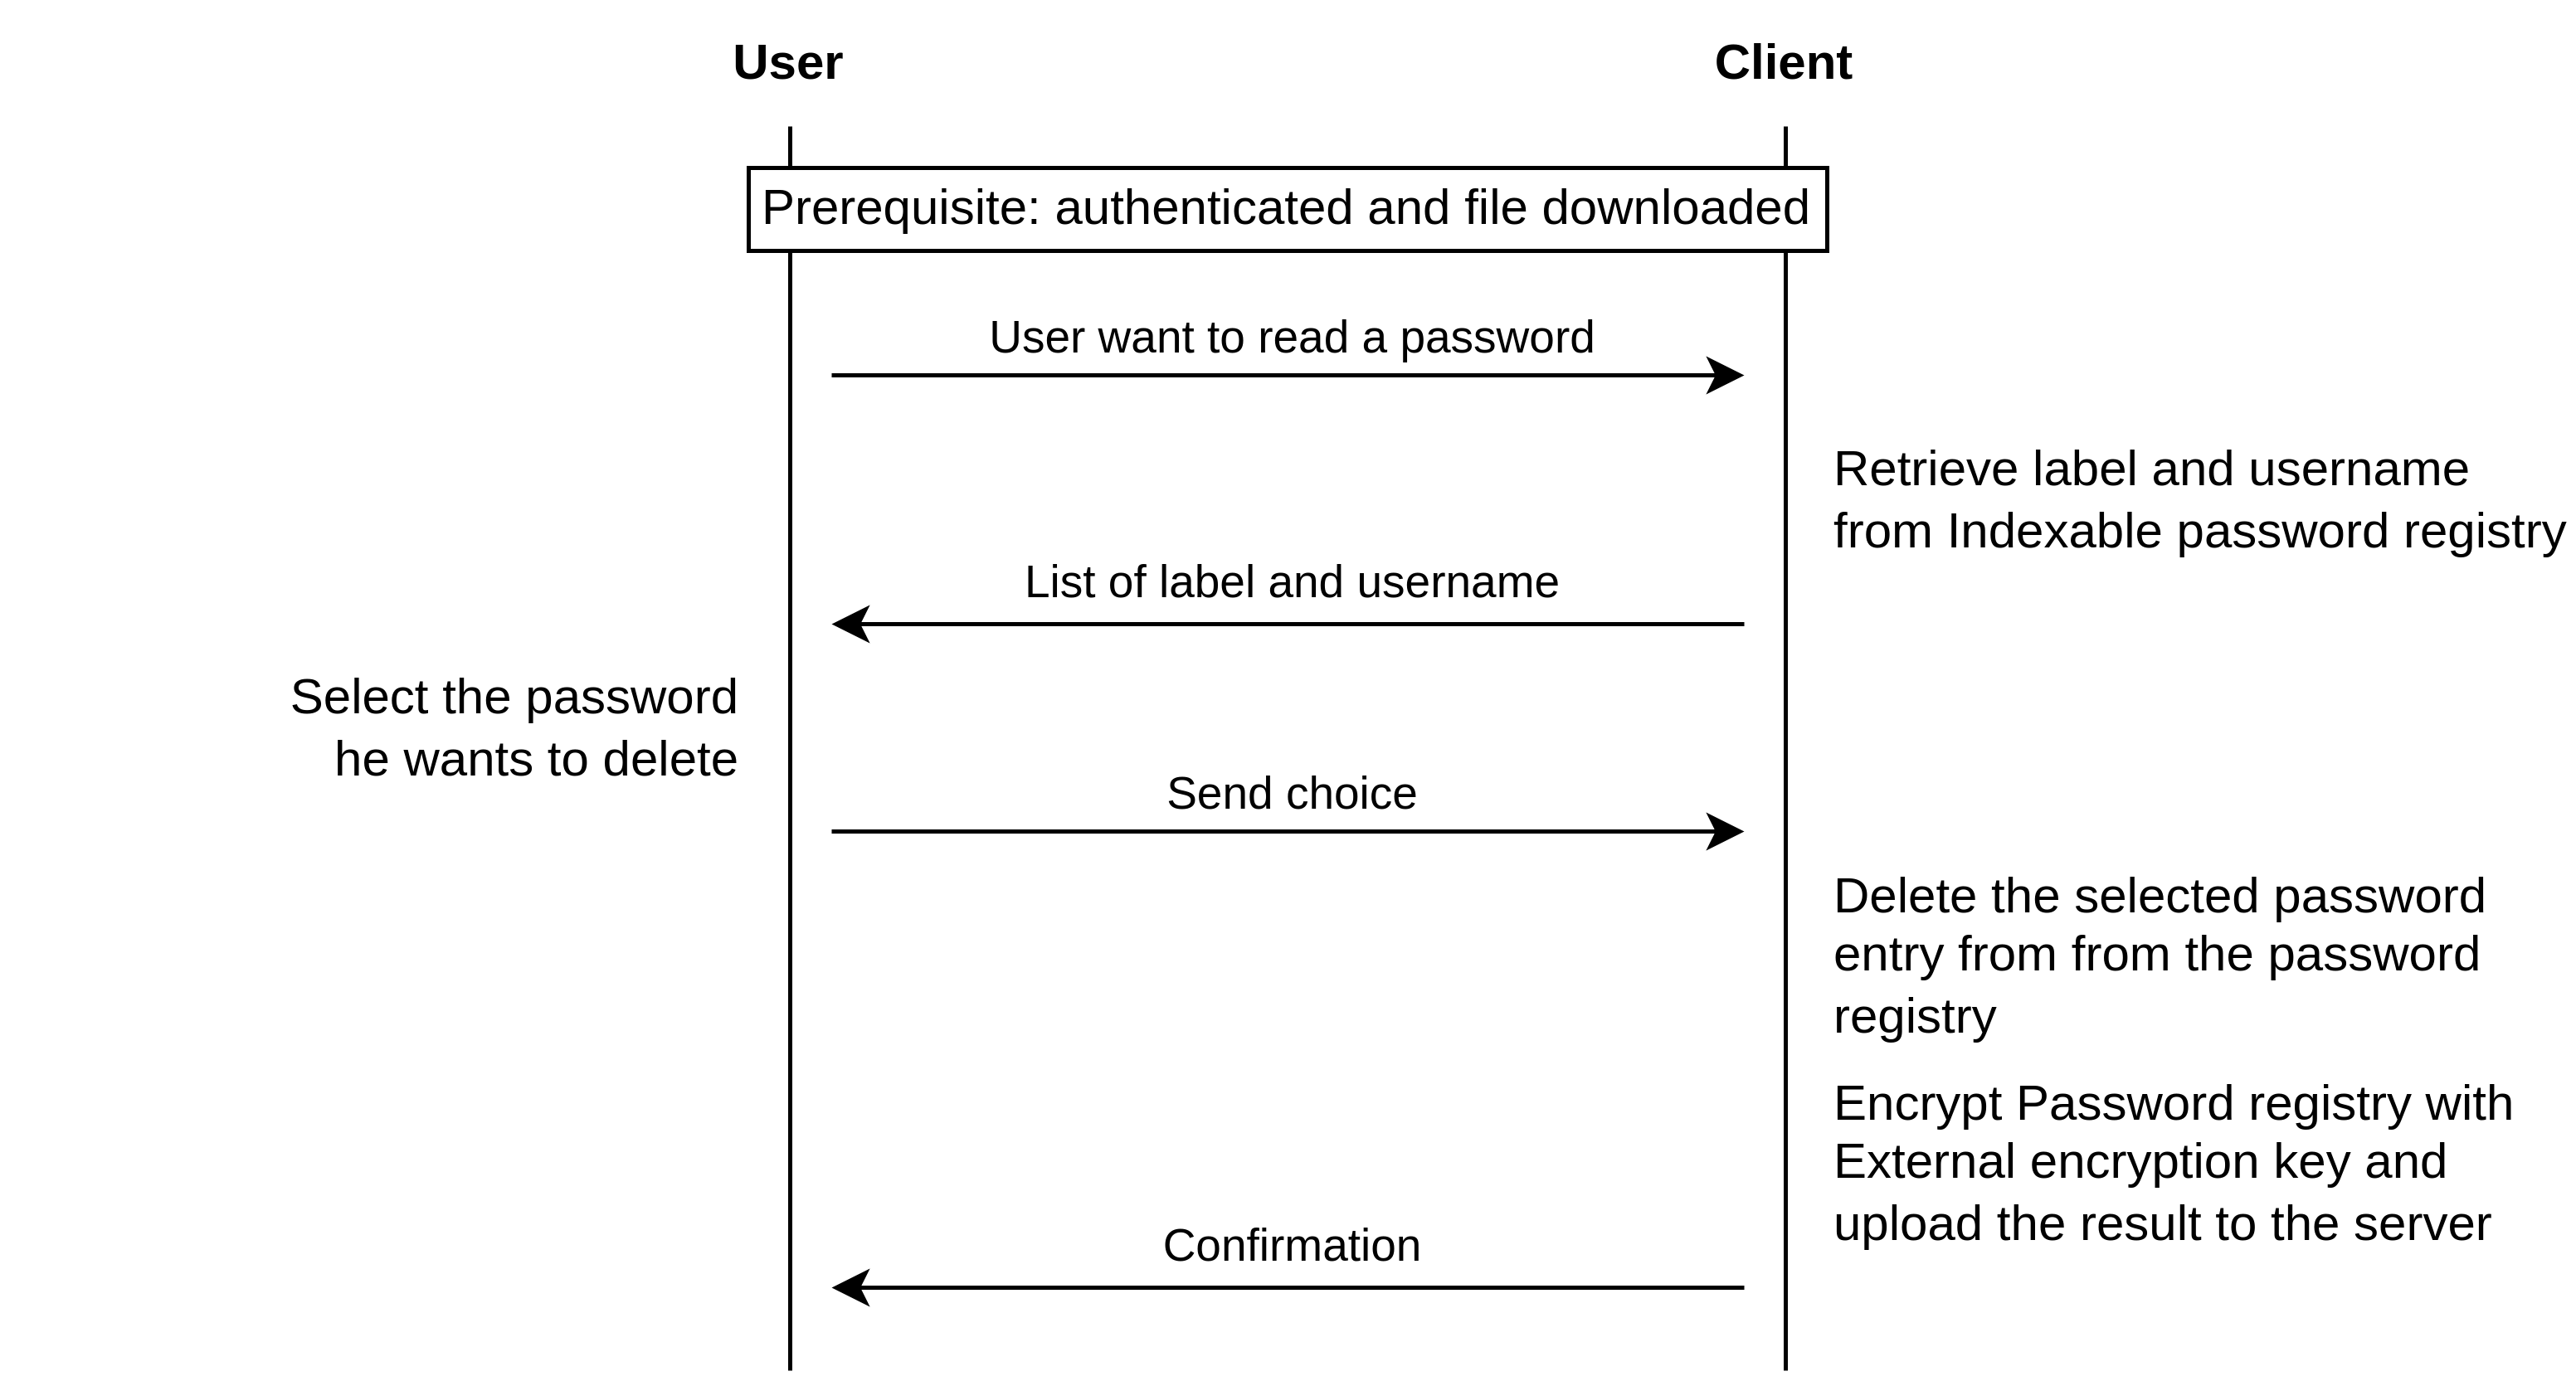
\includegraphics[width=\textwidth-22pt]{delete.png}}
 \caption{Interaction between the user and the client for deleting a password entry.}
 \label{fig:usecase_delete}
\end{figure}


\subsection{Advantages of KHAPE}
Using KHAPE for the authentication has two main advantages.
Firstly, and most importantly, it allows to authenticate the client to the server with a password without the password being ever visible to the server. As specified in the context section \ref{sec:usecase_context}, it is especially important for an application where the sensitive data is encrypted with a key that is also derived from the password.

Secondly, the utilization of the export key for the password registry decryption, make it more secure and more efficient.
More secure because computing an OPRF is more secure than just deriving a key in local since it forces the client to interact with the server. Only the server knows the secret salt used to compute the OPRF output. 
This mean that an attacker would be forced to compute online password guesses making it easier to mitigate by the server.

More efficient because KHAPE already compute an OPRF and a SlowHash for the authentication and derive multiple keys from the output --- including the export key.
If the export key was not provided to the application, the client would be forced to compute another SlowHash function on the password to derive a master key. This would drastically impact the performances of the application.


\subsection{Security considerations}
It is important to consider that even though each password is double encrypted, it is still possible to an attacker to retrieve all passwords. Since both the Indexable password registry and the Internal encryption key are kept in memory at rest, an attacker could dump the client's memory and derive every Individual password key to decrypt all passwords.
Mitigation to this would be to add a secret value to the Individual password key derivation. This secret value would be stored outside of the memory in a secure location such as an HSM or an Ubikey. This way, even if an attacker can dump the client's memory, he cannot derive any Individual password key and so he cannot retrieve any cleartext password. 

% \section{Implementation}
% At the moment, the implemented client is a CLI (command line interface)
% 
% The server is 
% - Server
% - database
% - no network
% 
% - taken from a project 
% - Currently the client is only CLI but planned to be compiled to wasm to be integrated to a browser
% - Server network is simulated.
% - Database
% - Github
% 
% - every transmission is secured
% - can use totp

\section{Implementation}
% - The implementation is functional (poc), rust (Github link)
% - Taken from a project 
% - Client is a CLI
% - Server implement use a sqlite database to store user's informations, encrypted user's data are stored in files
% - network is simulated
% 
% TODO : implement real network, compile in wasm to implement a browser client

The online password manager has been developed \footnote{Implementation can be found here : https://github.com/jul0105/OnlinePasswordManager} in Rust. It is a functional proof of concept that demonstrates the usefulness of KHAPE for such applications.
The implementation is based on an existing online password manager project that was developed earlier this year by Gil Balsiger and me.

Currently, the client is a CLI (command line interface). It is planned to be adapted
The server uses an SQLite database to store user information. Each user's encrypted data structure is stored on the server in a separated file. 
The network between the client and the server is simulated meaning that the client simply call server’s function instead of sending an actual TCP or HTTP request.

In the future, it is planned to adapt this prototype to be usable in practice. This will be done by implementing the network part. The client will also be adapted to compile the rust code in WebAssembly. The final goal is to build a client for web browsers.

\end{document}
